\documentclass[a4paper,10pt]{article} % article

\usepackage[english]{babel}
\usepackage{graphicx}
\usepackage{subfig}
\usepackage{amsmath}
\usepackage{amssymb}
\usepackage{hyperref}
\usepackage{doi}
\usepackage{mathtools}
\usepackage{anysize}
\usepackage{pgfplots}
\usetikzlibrary{arrows.meta}
\tikzset{myarrow/.style={-{Triangle[length=3mm,width=1mm]}}}
\marginsize{2cm}{2cm}{2cm}{2cm}

%Highligh code
% Custom colors
\usepackage{color}
\definecolor{deepblue}{rgb}{0,0,0.5}
\definecolor{deepred}{rgb}{0.6,0,0}
\definecolor{deepgreen}{rgb}{0,0.5,0}
\definecolor{codegreen}{rgb}{0,0.5,0.2}
\definecolor{backcolour}{rgb}{0.95,0.95,0.92}

\usepackage{listings}

\lstdefinestyle{mystyle}{
    backgroundcolor=\color{backcolour},
    commentstyle=\color{deepblue},
    keywordstyle=\color{codegreen},
    numberstyle=\tiny\color{deepgreen},
    stringstyle=\color{deepred},
    basicstyle=\footnotesize,
    breakatwhitespace=false,
    breaklines=true,
    captionpos=b,
    keepspaces=true,
    numbers=left,
    numbersep=5pt,
    showspaces=false,
    showstringspaces=false,
    showtabs=false,
    tabsize=2
}

\lstset{style=mystyle}

%Font
\usepackage{avant}
\usepackage[scaled]{helvet} % ss
\usepackage[helvet]{sfmath}
\normalfont
\renewcommand*\familydefault{\sfdefault} %% Only if the base font of the document is to be sans serif
\usepackage[T1]{fontenc}
\usepackage{type1cm}
\usepackage{courier}
\renewcommand{\ttdefault}{pcr}
\DeclareMathAlphabet\mathcal{OMS}{cmsy}{b}{n}

 %Head and foot page
\usepackage{fancyhdr}
\pagestyle{fancy}
\fancyhf{}
\fancyhead[L]{ContactStructuralMechanicsApplication}
\fancyhead[R]{ALMFrictionlessMortarCondition}
\fancyfoot[R]{\leftmark}
\fancyfoot[L]{\thepage}
\renewcommand{\headrulewidth}{0.4pt}
\renewcommand{\footrulewidth}{0.4pt}
% \renewcommand{\headwidth}{17cm}

\title{Augmented Lagrangian formulation for frictional contact based in \em{Mortar} integration}
\author{Vicente Mataix Ferr\'andiz}
\date{July 2018}

\pgfplotsset{compat=1.14}
\begin{document}

\maketitle

\section{Introduction}

The following document presents the formulation employed in the derivation of the frictional \textit{Mortar} contact condition formulation with augmented dual \textit{Lagrange multiplier} (\textbf{ADLM}), based in the work of \textit{Alexander Popp}\cite{popp1,popp2} and \textit{Alberto Cardona}\cite{cardona1,cardona2}. The contact mechanics problems are based on the \textbf{IBVP} of non-linear solid mechanics and the unilateral contact constraints. After recapitulating some basic notation and the strong formulation, a weak formulation of the contact mechanics problems with two subdomains will be introduced.  In contrast to the mesh tying case considered so far, unilateral contact leads to a constrained minimization problem with inequality constraints, or more generally to so-called variational inequalities. It should be mentioned that both frictionless and frictional contact can either be formulated as variational inequalities with
a constrained solution or as saddle point problems based on \textit{Lagrange multipliers}, where the focus will be on the latter approach here.

The motivation for dual \textit{Lagrange multipliers}\cite{wohlmuth} lies in the fact that an extension of the master side basis functions to the slave side of the interface has a global support for standard \textit{Lagrange multipliers}.

\section{Content}

\subsection{Frictionless contact}

Before introduce the formulation employed for the frictional contact, the formulation for the frictionless will be introduced. Many terms are reused and common in both formulation, so the theoretical introduction for the frictional case will require a smaller effort.

\subsubsection{Strong formulation}\label{section:stronfrictionless}

On each subdomain $\Omega_0^{(i)}$ , the initial boundary value problem of finite deformation elastodynamics needs to be satisfied, viz \eqref{eq:eq0}.

\begin{subequations}\label{eq:eq0}
\begin{align}
 & \text{Div} \mathbf{P}^{(i)}+\hat{\mathbf{b}}_0^{(i)}=\rho_0^{(i)}\ddot{\mathbf{u}}^{(i)} \text{ in } \Omega_0^{(i)} \times [0, T] \label{eq:subeq1}\\
 & \mathbf{u}^{(i)} = \hat{\mathbf{u}}^{(i)} \text{ on } \Gamma_u^{(i)} \times [0, T] \label{eq:subeq2}\\
 & \mathbf{P}^{(i)} \cdot \mathbf{N}^{(i)} = \hat{\mathbf{t}}_0^{(i)} \text{ on } \Gamma_\sigma^{(i)} \times [0, T] \label{eq:subeq3} \\
 & \mathbf{u}^{(i)}\left( \mathbf{X}^{(i)}, 0\right) = \hat{\mathbf{u}}_0^{(i)}\left( \mathbf{X}^{(i)}\right) \text{ in } \Omega_0^{(i)} \label{eq:subeq4} \\
 & \dot{\mathbf{u}}^{(i)}\left( \mathbf{X}^{(i)}, 0\right) = \hat{\dot{\mathbf{u}}}_0^{(i)}\left( \mathbf{X}^{(i)}\right) \text{ in } \Omega_0^{(i)} \label{eq:subeq5}
 \end{align}
\end{subequations}

The contact constraints in normal direction are typically given in form of \textit{Karush-Kuhn-Tucker}\textbf{KKT} conditions as given in \eqref{eq:eq6}, and Figure \ref{fig:kkt}.

 \begin{equation}\label{eq:eq6}
g_n \geq 0 \text{ , } p_n \leq 0 \text{ , } p_n g_n = 0 \text{ on } \Gamma_c^{(i)} \times [0, T]
 \end{equation}

\begin{figure}[h]
\begin{center}
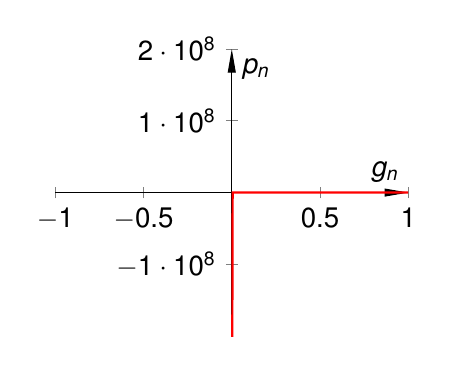
\begin{tikzpicture}
\begin{axis}[
%         grid= major ,
		width=0.5\textwidth ,
		xlabel style={font=\Large},
		xlabel = {$g_n$} ,
		ylabel style={font=\Large},
		ylabel = {$p_n$} ,
		xmin = -1,
		xmax = 1,
		ymin = -1,
		ymax = 1,
		axis lines=middle,
		axis line style={myarrow}
		]
\addplot[red, thick] expression[domain=-1:1, domain y=-1:1, samples=200] {(x>0? 0 : -10^9)};
\end{axis}
\end{tikzpicture}
\caption{\textit{Karush–Kuhn–Tucker} (\textbf{KKT}) conditions of non-penetration.}
\label{fig:kkt}
\end{center}
\end{figure}

In the course of deriving a weak formulation, the balance of linear momentum at the unilateral contact problem  for the interface $\Gamma_c^{(i)}$ is typically exploited and a \textit{Lagrange multiplier} vector field $\lambda_n$ is introduced, thus setting the basis for a mixed variational approach. Unilateral contact constraints are typically
formulated (and later also numerically evaluated) in the current configuration.

\subsubsection{Weak formulation}

\paragraph{Standard Lagrange multiplier}

To start the derivation of a weak formulation of \eqref{eq:eq0}, appropriate solution spaces $\mathcal{U}^{(i)}$ and
weighting spaces $\mathcal{V}^{(i)}$ need to be defined as \eqref{eq:eq7}.

\begin{equation}\label{eq:eq7}
 \begin{cases}
  \mathcal{U}^{(i)} = \left\{ \mathbf{u}^{(i)} \in H^1(\Omega) \| \mathbf{u}^{(i)} = \hat{\mathbf{u}}^{(i)} \text{ on } \Gamma_u^{(i)}\right\},\\
  \mathcal{V}^{(i)} = \left\{ \delta\mathbf{u}^{(i)} \in H^1(\Omega) \| \delta\mathbf{u}^{(i)} = \mathbf{0} \text{ on } \Gamma_u^{(i)}\right\}
 \end{cases}
\end{equation}

Additionally the \textit{Lagrange multiplier} vector $\boldsymbol{\lambda}_n = \lambda_n \cdot \mathbf{n} = -\mathbf{t}_c^{(1)}$, which enforce the unilateral contact constraint\eqref{eq:eq6}, represents the negative slave side contact traction $\mathbf{t}_c^{(1)}$, is chosen from a corresponding solution space denoted as $\mathcal{M}$.

In terms of its classification in functional analysis, this space represents the dual space of the trace space $\mathcal{W}^{(1)}$ of $\mathcal{V}^{(1)}$. In the given context, this means that $\mathcal{M} = H^{−1/2} (\Gamma_c)$ and $\mathcal{W}^{(1)} = H^{1/2} (\Gamma_c)$, where $\mathcal{M}$  and $\mathcal{W}^{(1)}$ denote single scalar components of the corresponding vector-valued spaces $\mathcal{M}$ and $\mathcal{W}$.

Based on these considerations, a saddle point type weak formulation is derived next. This can be done by extending the standard weak formulation of non-linear solid mechanics as defined to two subdomains and combining it with the \textit{Lagrange multiplier} coupling terms introduced in generic form. Find $\mathbf{u}^{(i)} \in \mathcal{U}^{(i)}$ and $\lambda_n \in \mathcal{M}$ such that we obtain \eqref{eq:eqfunct0}, than once derived \eqref{eq:eqfunct}.

\begin{subequations}
\begin{equation}\label{eq:eqfunct0}
\mathcal{W}^{co}(\mathbf{u},\lambda_n) = \int_{\Gamma_c^{(1)}} \lambda_n \cdot g_n \text{d}\Gamma_{co}^{(i)}
\end{equation}

Where $g_n$ is the continuous normal gap, that can be defined as \eqref{eq:eqgap}.

\begin{equation}\label{eq:eqgap}
 g_n = \mathbf{n}^{(1)}\cdot\left( \mathbf{u}^{(1)} - \mathbf{u}^{(2)}\right)
\end{equation}
\end{subequations}

\begin{subequations}\label{eq:eqfunct}
 \begin{align}
\delta\mathcal{W}(\mathbf{u},\lambda_n) = \delta\mathcal{W}_\mathcal{V} + \delta\mathcal{W}_\mathcal{M} & \\
\delta\mathcal{W}_\mathcal{V} = -\delta \mathcal{W}_{kin}(\mathbf{u}^{(i)},\delta \mathbf{u}^{(i)}) - \delta \mathcal{W}_{int,ext}(\mathbf{u}^{(i)},\delta \mathbf{u}^{(i)}) & - \delta\mathcal{W}_{co}(\boldsymbol{\lambda}^{(i)},\delta \mathbf{u}^{(i)}) = 0 \text{ } \forall \delta \mathbf{u}^{(i)} \in  \mathcal{V} \label{eq:subeq8} \\
\delta\mathcal{W}_\mathcal{M} = & - \delta\mathcal{W}_{\lambda}(\mathbf{u}^{(i)},\delta \boldsymbol{\lambda}^{(i)}) \geq 0 \text{ } \forall \delta \boldsymbol{\lambda}^{(i)} \in  \mathcal{M} \label{eq:subeq9}
 \end{align}
\end{subequations}

Herein, the kinetic contribution $\delta \mathcal{W}_{kin}$ , the internal and external contributions $\delta \mathcal{W}_{int,ext}$ and the unilateral contact contribution $\delta\mathcal{W}_{co}$ to the overall virtual work on the two subdomains, as well as the weak form of the unilateral contact constraint $\delta\mathcal{W}_{\lambda}($, have been abbreviated as \eqref{eq:constributions}.

\begin{subequations}\label{eq:constributions}
 \begin{align}
  & -\delta \mathcal{W}_{kin} = \sum_{i = 1}^2 \left[\int_{\Omega_0^{(i)}} \rho_0^{(i)} \ddot{\mathbf{u}}^{(i)} \cdot \delta \mathbf{u}^{(i)} \text{d}\Omega_{0}^{(i)}\right] \label{eq:subeq10} \\
 & -\delta \mathcal{W}_{int,ext} = \sum_{i = 1}^2 \left[\int_{\Omega_0^{(i)}} \left(\mathbf{S}^{(i)} : \delta \mathbf{E}^{(i)} - \hat{\mathbf{b}}\cdot \delta\mathbf{u}^{(i)} \right) \text{d}\Omega_{0}^{(i)} - \int_{\Gamma_\sigma^{(i)}} \hat{\mathbf{t}}_0^{(i)}\cdot\delta\mathbf{u}^{(i)} \text{d}\Gamma_{\sigma}^{(i)} \right] \label{eq:subeq11} \\
 & -\delta \mathcal{W}_{co} = \sum_{i = 1}^2 \left[\int_{\Gamma_c^{(i)}} \lambda_n \cdot \delta g_n \text{d}\Gamma_{co}^{(i)}\right] \label{eq:subeq12} \\
 & -\delta \mathcal{W}_{\lambda} = \sum_{i = 1}^2 \left[\int_{\Gamma_c^{(i)}} \delta \lambda_n \cdot g_n \text{d}\Gamma_{co}^{(i)}\right] \label{eq:subeq13}
 \end{align}
\end{subequations}

The coupling terms on $\Gamma_c$ also allow for a direct interpretation in terms of variational formulations and the principle of virtual work. Whereas the contribution in \eqref{eq:subeq12} represents the virtual work of the unknown interface tractions $\boldsymbol{\lambda} = −\mathbf{t}_c^{(1)} = \mathbf{t}_c^{(2)}$, the contribution in \eqref{eq:subeq13} ensures a weak, variationally consistent enforcement of the unilateral contact constraint \eqref{eq:eq6}. Nevertheless, the concrete choice of the discrete Lagrange multiplier space $\mathcal{M}_h$ in the context of mortar finite element discretisations is decisive for the stability of the method and for optimal a priori error bounds. Finally, it is pointed out that the weak formulation \eqref{eq:subeq8} and \eqref{eq:subeq9} possesses all characteristics of saddle point problems and \textit{Lagrange multiplier} methods.

In contrast to the mesh tying case, where this mapping only came into play in the discrete setting, $\gamma_c^{(1)}$ and $\gamma_c^{(2)}$ cannot even be guaranteed to be identical in the continuum framework for unilateral contact, because they not only comprise the actual contact surfaces but the potential contact surfaces.

As compared with the mesh tying case, it is noticeable that the weak formulation contains inequality \eqref{eq:subeq9} conditions for unilateral contact. These require a particular numerical treatment based on active set strategies.

\paragraph{Augmented Lagrange multiplier}

One of the main disadvantages of the standard \textit{Lagrange multiplier} is the saddle point problem that appears in the formulation. For solving that, an \textbf{Augmented Lagrangian} method to solve contact problems with friction was proposed by \textit{Alart and Curnier}\cite{alart} based on a reformulation of the contact and friction laws into a system
of equations without inequalities.

Focusing in the functional relative to the contact ($\mathcal{W}^{co}(\mathbf{u},\lambda_n) = \mathcal{W}^{co}_\mathcal{V} + \mathcal{W}_\mathcal{M}$), we can rewrite \eqref{eq:eqfunct0} as \eqref{eq:eqalmfunct0}.

\begin{equation}\label{eq:eqalmfunct0}
 \mathcal{W}^{co}(\mathbf{u},\lambda_n) = \int_{\Gamma_c^{(1)}} k \lambda_n \cdot g_n  + \frac{\varepsilon}{2} g_n^2 - \frac{1}{2\varepsilon} \langle k \lambda_n + \varepsilon g_n \rangle^2\text{d}\Gamma_{co}^{(i)}
\end{equation}

Where $\varepsilon$ is a positive penalty parameter, $k$ is a positive scale factor, and $\langle \rangle$ is the \textit{Macauley} bracket operator, that is \eqref{eq:eqmac}.

\begin{equation}\label{eq:eqmac}
 \langle x \rangle \begin{cases} x \text{ } x \geq 0\\ 0 \text{ } x < 0 \end{cases}
\end{equation}

This functional is $\mathcal{C}^1$ differentiable saddle-point, as shown in Figure \ref{fig:locusalm}. The solution is obtained as the set of values that render this functional stationary.

\begin{figure}[h]
\begin{center}
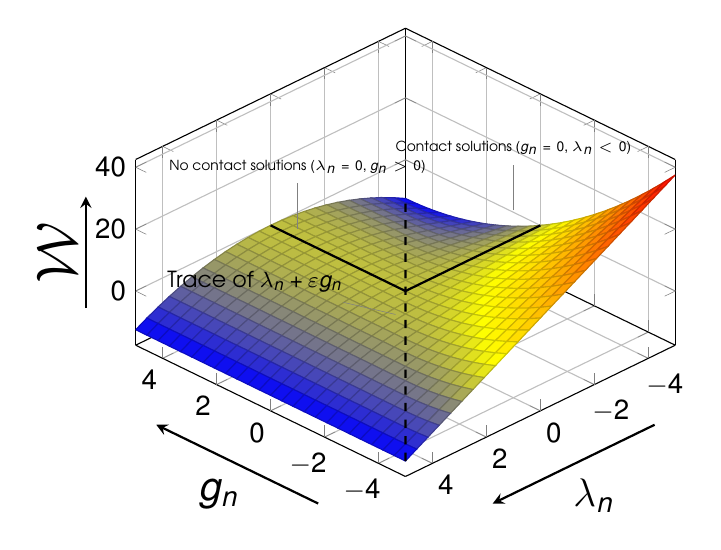
\begin{tikzpicture}[
declare function={functional(\r,\k)={(\k*y+\r*x > 0 ? \k*y*x+\r*0.5*x^2-0.5/\r*(\k*y+\r*x)^2:\k*y*x+\r*0.5*x^2)};}
]
\begin{axis}[grid=both,
%             title= Augmented Lagrangian function for the contact problem,
            xlabel={$g_n$},
            xticklabel pos=left,
            xlabel style={font=\Large},
            ylabel={$\lambda_n$},
            x dir=reverse,
            yticklabel pos=left,
            ylabel style={font=\Large},
            y dir=reverse,
            zlabel={$\mathcal{W}$},
            zticklabel pos=left,
            zlabel style={font=\huge},
            after end axis/.code={
                \draw [-stealth, thick, black] (xticklabel cs:0.8) -- (xticklabel cs:0.2);
                \draw [-stealth, thick, black] (yticklabel cs:0.8) -- (yticklabel cs:0.2);
                \draw [-stealth, thick, black] (zticklabel cs:0.2) -- (zticklabel cs:0.8);
            }
            ,unbounded coords = jump
            ,view = {45}{45}
%             ,colormap name  = whitered
%             ,colorbar style = {
%                 at     = {(1,0)},
%                 anchor = south west,
%                 height = 0.25*\pgfkeysvalueof{/pgfplots/parent axis height},
%                 title  = {$\mathcal{W}$}
%                 }
            ]
\addplot3[surf,shader=faceted]{functional(1.0,1.0)};
\addplot3[samples=30,samples y=0, thick, dashed ,black,smooth]({x},{-x},{-0.5*x^2});
\addplot3[samples=30, domain=5:0, samples y=0, thick,black,smooth]({x},{0.0},{0.0});
\addplot3[samples=30, domain=0:-5,samples y=0, thick,black,smooth]({0.0},{x},{0.0});
\node at (axis cs: 4.0,0.0,0.0 ) [pin=90:\tiny{No contact solutions  $(\lambda_n=0,g_n>0)$}] {};
\node at (axis cs: 0.0,-4.0,6.0) [pin=90:\tiny{Contact solutions $(g_n=0,\lambda_n<0)$}] {};
\node at (axis cs:-1,1,0.18) [pin=165:\footnotesize{Trace of $\lambda_n+\varepsilon g_n$}] {};
\end{axis}
\end{tikzpicture}
\caption{Augmented Lagrangian function for the contact problem. The locus of solutions is displayed.}
\label{fig:locusalm}
\end{center}
\end{figure}

The solution does not depend on the value of parameters $\varepsilon$ and $k$. Nevertheless, the convergence rate does depend on their value. In numerical computations, default values of $\varepsilon$ and $k$ are selected in terms of a mean value of the \textit{Young} modulus of the bodies in contact and of a mean value of mesh size, as \eqref{eq:eqcoeff}. Numerical examples show that this choice gives a better condition number of the iteration matrix than other choices.

\begin{equation}\label{eq:eqcoeff}
 \varepsilon = k \approx 10 \frac{E_{mean}}{h_{mean}}
\end{equation}

The functional \eqref{eq:eqalmfunct0} can be separated in two different parts, as can be seen in \eqref{eq:eqalmfunct1}.

\begin{equation}\label{eq:eqalmfunct1}
  \mathcal{W}^{co}(\mathbf{u},\lambda_n) = \int_{\Gamma_c^{(1)}} \begin{cases}  k \lambda_n \cdot g_n  + \frac{\varepsilon}{2} g_n^2 \text{d}\Gamma_{co}^{(i)} & \text{ if } k\lambda_n +\varepsilon g_n \leq 0 \text{ (Contact zone)} \\ - \frac{k}{2\varepsilon} \lambda_n^2   & \text{ if } k\lambda_n +\varepsilon g_n > 0 \text{ (Gap zone)} \end{cases}\text{d}\Gamma_{co}^{(i)}
\end{equation}

Finally we can derive \eqref{eq:eqalmfunct1} to obtain the variational form from \eqref{eq:eqalmfunct2}, where to simplify we define the augmented normal pressure $\hat{\lambda}_{n} = k\lambda_n +\varepsilon g_n $.

\begin{equation}\label{eq:eqalmfunct2}
  \delta \mathcal{W}^{co}(\mathbf{u},\lambda_n) = \int_{\Gamma_c^{(1)}}\begin{cases}  \hat{\lambda}_{n} \cdot \delta g_n + k g_n \delta\lambda_n & \text{ if } \hat{\lambda}_{n} \leq 0 \text{ (Contact zone)} \\  - \frac{k^2}{\varepsilon} \lambda_n \delta\lambda_n & \text{ if } \hat{\lambda}_{n} > 0 \text{ (Gap zone)} \end{cases} \text{d}\Gamma_{co}^{(i)}
\end{equation}

The functional from \eqref{eq:eqalmfunct2} makes that the system obtained varies in function if the nodes are present in the contact or the gap zone, so the system is not a priori known and in the following to present the numerical discretisation will focus in the solution obtained in the gap zone. Once this is derived the solution in the gap zone can be obtained in a in a straight-forward way.

\subsubsection{Discretisation and numerical integration}

\paragraph{Dual Lagrange multipliers}

\subparagraph{Definition}:

The discretisations of the displacements correspond with the standard ones in the finite element formulation, for more information check the literature\cite{Zienkiewicz1}. In addition, an adequate discretisation of the Lagrange multiplier vector $\boldsymbol{\lambda}$ is needed, and will be based on a discrete \textit{Lagrange multiplier} space $\mathcal{M}_h$ being an approximation of $\mathcal{M}$. Thus, we can define the discete \textit{Lagrange multiplier} as \eqref{eq:eq14}, with the shape functions $\Phi_j$ and the discrete nodal Lagrange multipliers $\boldsymbol{\lambda}_h$.

\begin{equation}\label{eq:eq14}
 \boldsymbol{\lambda}_h = \sum_{i=1}^{m^{(1)}} \Phi_j\left(\xi^{(1)},\eta^{(1)} \right) \boldsymbol{\lambda}_j
\end{equation}

Details on how to define dual Lagrange multiplier shape functions $\Phi_j$ using the so-called biorthogonality relationship with the standard displacement shape functions $N_k$ have first been presented in \textit{Wohlmuth}\cite{wohlmuth}. A common notation of the biorthogonality condition is \eqref{eq:eq15}.

\begin{equation}\label{eq:eq15}
 \int_{\Gamma_{co,h}^{(1)}}\Phi_j N_k^{(1)} \text{d}\Gamma_{co}^{(i)} = \delta_{jk} \int_{\Gamma_{co,h}^{(1)}} N_k^{(1)} \text{d}\Gamma_{co}^{(i)} \text{ , } j,k=1,...,m^{(1)}
\end{equation}

Herein, $\delta_{jk}$ is the \textit{Kronecker} delta, and the most common choice $m^{(1)} = n^{(1)}$ is assumed. For
practical reasons, the biorthogonality condition is typically applied locally on each slave element $e$, yielding \eqref{eq:eq16}, where $m_e^{(1)}$ represents the number of Lagrange multiplier nodes of the considered slave element.

\begin{equation}\label{eq:eq16}
 \int_{e}\Phi_j N_k^{(1)} \text{d}e = \delta_{jk} \int_{e} N_k^{(1)} \text{d}e \text{ , } j,k=1,...,m_e^{(1)}
\end{equation}

Combining the biorthogonality condition in \eqref{eq:eq16} and the partition of unity property of the dual shape functions, it follows that \eqref{eq:eq17}.

\begin{equation}\label{eq:eq17}
 \int_e \Phi_j de =  \int_e N_j^{(1)} de \text{ , } j=1,...,m_e^{(1)}
\end{equation}

It is important to point out that the element-wise biorthogonality condition in \eqref{eq:eq16} must be satisfied in the physical space, and not simply in the finite element parameter space. Consequently, a matrix system of size $m_e^{(1)} \times m_e^{(1)}$ must be solved on each slave element. The first step for doing this is to introduce unknown linear coefficients $a_{jk}$ such that \eqref{eq:eq18}.

\begin{equation}\label{eq:eq18}
 \Phi_j(\xi, \eta) = a_{jk} N_k^{(1)}\left(\xi, \eta \right), \mathbf{A}_e = [a_{jk}] \in \mathbb{R}^{m_e^{(1)} \times m_e^{(1)}}
 \end{equation}

 It can easily be verified that, as second step, insertion of \eqref{eq:eq18} into \eqref{eq:eq16} yields the unknown
coefficient matrix $\mathbf{A}_e$ as \eqref{eq:eq19}, where $J(\xi, \eta)$ is the slave \textit{Jacobian} determinant.

\begin{equation}\label{eq:eq19}
\begin{aligned}
 & \mathbf{A}_e = \mathbf{D}_e\mathbf{M}_e^{-1} \\
 & \mathbf{D}_e = [d_{jk}] \in \mathbb{R}^{m_e^{(1)} \times m_e^{(1)}}, d_{jk} = \delta_{jk} \int_e N_k^{(1)}(\xi, \eta) J(\xi, \eta) \text{d}e \\
 & \mathbf{M}_e = [m_{jk}] \in \mathbb{R}^{m_e^{(1)} \times m_e^{(1)}}, m_{jk} = \int_e N_j^{(1)}(\xi, \eta) N_k^{(1)}(\xi, \eta) J(\xi, \eta) \text{d}e
\end{aligned}
 \end{equation}

\subparagraph{Derivatives}:

To define $\Delta \phi$ it is necessary to define the derivatives from \eqref{eq:eq19}, which can be obtained with \eqref{eq:eq19b}.

\begin{equation}\label{eq:eq19b}
\begin{aligned}
 & \Delta \mathbf{A}_e = \Delta \mathbf{D}_e\mathbf{M}_e^{-1} - \mathbf{D}_e\Delta\mathbf{M}_e\mathbf{M}_e^{-1} \\
 &\Delta \mathbf{D}_e = \Delta[d_{jk}] \in \mathbb{R}^{m_e^{(1)} \times m_e^{(1)}}, \Delta d_{jk} = \delta_{jk} \sum_{g = 1}^{n_{gp}} w_g N_{gk}^{(1)} \Delta J_g^{(1)}  \\
 & \Delta \mathbf{M}_e = \Delta[m_{jk}] \in \mathbb{R}^{m_e^{(1)} \times m_e^{(1)}}, \Delta m_{jk} = \sum_{g = 1}^{n_{gp}} w_g  \sum_{g = 1}^{n_{gp}} w_g  N_{gj}^{(1)} N_{gk}^{(1)} \Delta J_g^{(1)}
\end{aligned}
 \end{equation}

\paragraph{Mortar operators}\label{section:mortar}

\subparagraph{Definition}:

Considering the discrete \textit{Lagrange multiplier}\eqref{eq:eq14} in \eqref{eq:subeq8} we obtain \eqref{eq:eq20}, where $\chi_h$ is the interface mapping.

\begin{equation}\label{eq:eq20}
 -\delta \mathcal{W}_{co,h} = \sum_{j=1}^{m^{(1)}}\sum_{k=1}^{n^{(1)}} \boldsymbol{\lambda}_{nj}^T \left(\int_{\Gamma_{c,h}^{(1)}} \Phi_j N_k^{(1)} \text{d}\Gamma_{co}^{(i)} \right) \delta \mathbf{d}_{nk}^{(1)} -\sum_{j=1}^{m^{(1)}}\sum_{l=1}^{n^{(2)}} \boldsymbol{\lambda}_{nj}^T \left(\int_{\Gamma_{c,h}^{(1)}} \Phi_j \left(N_l^{(2)} \circ \chi_h\right) \text{d}\Gamma_{co}^{(i)} \right) \delta \mathbf{d}_{nl}^{(2)}
\end{equation}

Numerical integration of the mortar coupling terms is exclusively performed on the slave side $\Gamma_{c,h}$ of the interface. In \eqref{eq:eq20}, nodal blocks of the two mortar integral matrices commonly denoted as $\mathbf{D}$ and $\mathbf{M}$ can be identified. This leads to the following definitions \eqref{eq:eq21}.

 \begin{equation}\label{eq:eq21}
 \begin{aligned}
 & \mathbf{D}[j,k] = D_{jk} \mathbf{I}_{ndim} = \int_{\Gamma_{c,h}^{(1)}} \Phi_j N_k^{(1)}\text{d}\Gamma_{co}^{(i)}\mathbf{I}_{ndim}\text{ , } j=1,...m^{(1)}\text{ , } k= 1, ...n^{(1)} = \sum_{g = 1}^{n_{gp}} w_g \phi_{gj} N_{gk}^{(1)} J_g^{(1)} \\
 & \mathbf{M}[j,l] = M_{jl} \mathbf{I}_{ndim} = \int_{\Gamma_{c,h}^{(1)}} \Phi_j \left(N_l^{(2)} \circ \chi_h \right)\text{d}\Gamma_{co}^{(i)}\mathbf{I}_{ndim}\text{ , } j=1,...m^{(1)}\text{ , } k= 1, ...n^{(2)} = \sum_{g = 1}^{n_{gp}} w_g \phi_{gj} N_{gk}^{(2)} J_g^{(1)}
 \end{aligned}
\end{equation}

Wit these matrices we can express the functional \eqref{eq:eq20} in the following way \eqref{eq:eq22}.

\begin{equation}\label{eq:eq22}
 -\delta \mathcal{W}_{co,h} = \delta \mathbf{x}_{n\mathcal{S}}^T\mathbf{D}^T\lambda_n - \delta \mathbf{x}_{n\mathcal{M}}^T\mathbf{M}^T\lambda_n = \delta \mathbf{x}_n \underbrace{\left[\begin{array}{c} \mathbf{0} \\ -\mathbf{M}^T \\ \mathbf{D}^T\end{array} \right]}_{\mathbf{B}^T_{co}} \lambda_n = \delta \mathbf{x}_n^T \mathbf{f}_{co}(\lambda_n)
\end{equation}

Herein, the discrete mortar unilateral contact operator $\mathbf{B}_{co}$ and the resulting discrete vector of unilateral contact forces $\mathbf{f}_{co} (\lambda_n) = \mathbf{B}_{co}\lambda_n$ acting on the slave and the master side of the interface are introduced.

To finalise the discretisation of the considered unilateral contact problem, a closer look needs to
be taken at the weak constraint contribution $\delta \mathcal{W}_{\lambda,h} $ in \eqref{eq:subeq9}. Due to the saddle point characteristics and resulting symmetry of the mixed variational formulation in \eqref{eq:subeq8}  and \eqref{eq:subeq9}, all discrete components of $\delta \mathcal{W}_{\lambda,h}$ have already been introduced and the final formulation is given as \eqref{eq:eq23}, with $\mathbf{g}_{n}(\mathbf{x}) = \mathbf{B}_{mt} \mathbf{x} \cdot \mathbf{n}$ representing the discrete unilateral contact constraint at the coupling interface.

\begin{equation}\label{eq:eq23}
 -\delta \mathcal{W}_{\lambda,h} = \delta \lambda_n^T\mathbf{D}\mathbf{x}_{n\mathcal{S}} - \delta \lambda_n^T\mathbf{M}\mathbf{x}_{n\mathcal{M}}= \delta \lambda_n^T \mathbf{B}_{mt} \mathbf{x} \cdot \mathbf{n} = \delta \lambda_n^T \mathbf{g}_{n}(\mathbf{x})
\end{equation}

This discrete form of $\mathbf{g}_{n}$ can be renamed as nodal weighted gap for each node ($\tilde{g}_n$).

\subparagraph{Derivatives}:

To obtain a fully quadratic convergence in the computation of the contact problem we should compute the derivatives of the \textit{Mortar} operators, in consequence the derivatives of the \textit{Mortar} operators can be defined as \eqref{eq:eq24}.

\begin{subequations}\label{eq:eq24}
\begin{equation}
 \begin{aligned}
 \Delta\mathbf{D}[j,k] & = \Delta D_{jk} \mathbf{I}_{ndim} = \Delta  \int_{\Gamma_{c,h}^{(1)}} \Phi_j N_k^{(1)}\text{d}\Gamma_{co}^{(i)}\mathbf{I}_{ndim}\text{ , } j=1,...m^{(1)}\text{ , } k= 1, ...n^{(1)} \\
 & = \sum_{g = 1}^{n_{gp}} w_g \Delta\phi_{gj}        N_{gk}^{(1)}        J_g^{(1)} + \sum_{g = 1}^{n_{gp}} w_g       \phi_{gj} \Delta N_{gk}^{(1)}        J_g^{(1)} + \sum_{g = 1}^{n_{gp}} w_g        \phi_{gj}       N_{gk}^{(1)} \Delta J_g^{(1)}
 \end{aligned}
 \end{equation}
 \begin{equation}
 \begin{aligned}
 \Delta\mathbf{M}[j,l]  & = \Delta M_{jl} \mathbf{I}_{ndim}  = \Delta  \int_{\Gamma_{c,h}^{(1)}} \Phi_j \left(N_l^{(2)} \circ \chi_h \right)\text{d}\Gamma_{co}^{(i)}\mathbf{I}_{ndim}\text{ , } j=1,...m^{(1)}\text{ , } k= 1, ...n^{(2)} \\
 & = \sum_{g = 1}^{n_{gp}} w_g \Delta\phi_{gj}        N_{gk}^{(2)}        J_g^{(1)}  + \sum_{g = 1}^{n_{gp}} w_g       \phi_{gj} \Delta N_{gk}^{(2)}        J_g^{(1)}  + \sum_{g = 1}^{n_{gp}} w_g        \phi_{gj}       N_{gk}^{(2)} \Delta J_g^{(1)}
 \end{aligned}
 \end{equation}
\end{subequations}

\paragraph{Matrix form of the problem}

\textcolor{red}{Complete with all the casuistry }

Finally, once computed the mortar operators, the resulting system for unilateral contact corresponds (for fully activated system) with \eqref{eq:eq24}.

\begin{equation}\label{eq:eq24}
 \left[ \begin{array}{cccc} \mathbf{K}_{\mathcal{N}\mathcal{N}} &  \mathbf{K}_{\mathcal{N}\mathcal{M}} & \mathbf{K}_{\mathcal{N}\mathcal{S}} & \mathbf{0} \\ \mathbf{K}_{\mathcal{N}\mathcal{N}}  & \mathbf{K}_{\mathcal{M}\mathcal{M}} & \mathbf{0} & -(\mathbf{M}\cdot \mathbf{n})^{T} \\ \mathbf{K}_{\mathcal{S}\mathcal{N}} & \mathbf{0} & \mathbf{K}_{\mathcal{S}\mathcal{S}} & (\mathbf{D}\cdot \mathbf{n})^T \\ \mathbf{0} & -(\mathbf{M}\cdot \mathbf{n}) & (\mathbf{D}\cdot \mathbf{n}) & \mathbf{0}   \end{array} \right] \left[ \begin{array}{c} \Delta\mathbf{d}_{\mathcal{N}} \\ \Delta\mathbf{d}_{\mathcal{M}} \\ \Delta\mathbf{d}_{\mathcal{S}} \\ \Delta\lambda_n \end{array} \right] = - \left[ \begin{array}{c} \mathbf{r}_{\mathcal{N}} \\ \mathbf{r}_{\mathcal{M}} \\ \mathbf{r}_{\mathcal{S}} \\ g_n \end{array} \right]
\end{equation}

\subsubsection{Active set strategy (Semismoth Newton Raphson)}

As mentioned before, the fully discrete problem statement of unilateral contact causes one major additional complexity with regard to global solution schemes as compared with the mesh tying case, namely the contact specific inequality constraints, which divide the set of all discrete constraints into two a priori unknown sets of active and inactive constraints. Mathematically speaking, this introduces an additional source of non-linearity apart from the well-known geometrical and material non-linearities of non-linear solid mechanics. To resolve this contact non-linearity, so-called primal-dual active set strategies (\textbf{PDASS}) will be employed.

The idea of any active set strategy in the context of unilateral contact is to find the correct subset of all slave nodes which are in contact with the master surface at the end of the currently considered time interval. The \textbf{PDASS} in  suffers from a serious drawback: the contact non-linearity, finding the correct active set A can not be resolved by a \textit{Newton–Raphson} type approach.

The basic idea of an alternative \textbf{PDASS} formulation is to re-arrange the \textbf{KKT} conditions such that a \textit{Newton–Raphson} type algorithm can be applied not only for geometrical and material non-linearities, but also for the non-linearity stemming from contact itself, i.e. the active set search. So we reformulate the discrete \textbf{KKT} conditions within a so-called non-linear complementarity (\textbf{NCP}) function (Figure \ref{fig:ncp}). This function in the case of frictionless case basically corresponds with the augmented normal contact pressure $\hat{\boldsymbol{\lambda}}_n$ presented before, and the criteria will be to activate/inactivate the corresponding node when the augmented contact pressure is in compression or traction correspondingly.

\begin{figure}[h]
\begin{center}
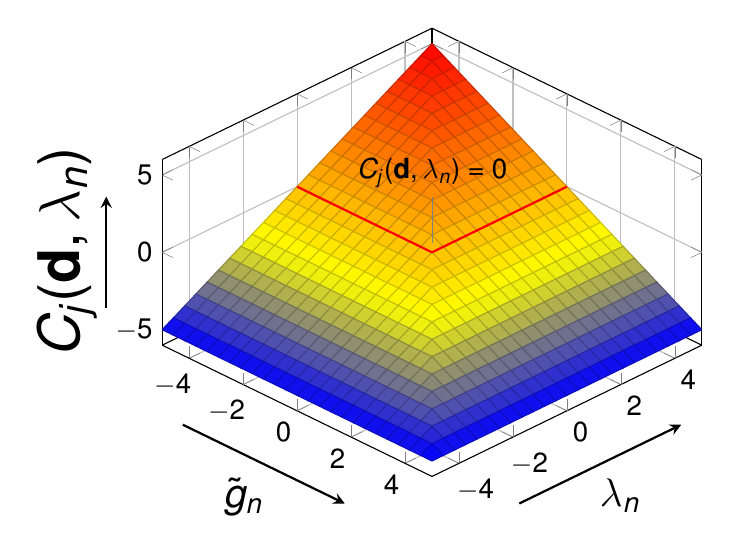
\begin{tikzpicture}[
declare function={myfunction(\r,\k)={\k*y - max(0, \k*y+\r*x)};}
]
\begin{axis}[grid=both,
            xlabel={$\tilde{g}_n$},
            xticklabel pos=left,
            xlabel style={font=\Large},
            ylabel={$\lambda_n$},
            yticklabel pos=left,
            ylabel style={font=\Large},
            zlabel={$C_j(\mathbf{d}, \lambda_n)$},
            zticklabel pos=left,
            zlabel style={font=\huge},
            after end axis/.code={
                \draw [-stealth, thick, black] (xticklabel cs:0.2) -- (xticklabel cs:0.8);
                \draw [-stealth, thick, black] (yticklabel cs:0.2) -- (yticklabel cs:0.8);
                \draw [-stealth, thick, black] (zticklabel cs:0.2) -- (zticklabel cs:0.8);
            }
            ,unbounded coords = jump
            ,view = {45}{45}
            ]
\addplot3[surf,shader=faceted]{myfunction(1.0,1.0)};
\addplot3[samples=30, domain=-5:0, samples y=0, thick,red,smooth]({x},{0.0},{0.0});
\addplot3[samples=30, domain= 0:5,samples y=0, thick,red,smooth]({0.0},{x},{0.0});
\node at (axis cs: 0.0,0.0,0.0 ) [pin=90:\normalsize{$C_j(\mathbf{d}, \lambda_n) = 0$}] {};
\end{axis}
\end{tikzpicture}
\caption{Exemplary nodal \textbf{NCP} function $\hat{\boldsymbol{\lambda}}_n$ the normal part of the nodal weighted
gap $\tilde{g}_n$ and the nodal normal contact pressure $\lambda_n$. The equivalence with the \textbf{KKT} conditions is indicated in red colour.
}
\label{fig:ncp}
\end{center}
\end{figure}

Thus, the resulting \textbf{PDASS} contains derivative information on the sets themselves and allows for the application of a \textit{Newton–Raphson} type solution scheme also for the non-linearity stemming from contact. Consequently, all sources of non-linearities, i.e. finite deformations, non-linear material behaviour and contact itself, can be treated
within one single iterative scheme.

\subsection{Frictional contact}

In the same manner to the frictionless case before introduce the weak formulation we need to formulate the problem we require the definition of the strong formulation. The formulation is a combination of the following references \cite{cardona3, gitt1, doca1, doca2, laursen2}.

\subsubsection{Strong formulation}

The part relative to the solutions spaces is exactly the same than the one presented for the frictionless case \eqref{eq:eq7} as well as the balance of the linear momentum \eqref{eq:eq0}. The \textbf{KKT} (\ref{section:stronfrictionless}) condition is still into play for the frictional problem.

\paragraph{Tangential contact condition - \textit{Coulomb's law}}

Friction is a complex physical phenomenon. The science that studies the friction, the tribology, has concluded the many origins of the physics of the frictional phenomenons. This combines the interactions of elastic and plastic deformations at the contact interface, interaction with wear particles, microfractures, excitation of electrons, etcetera. In continuum mechanics, the most common description is the phenomenological, or macroscopic, law of \textit{Coulomb} (Figure \ref{fig:coulomb}), which with \textit{Tresca}\footnote{Which is simpler because does not depend on contact normal pressure.} are the most extended and yet simple models of friction.

\begin{figure}[h]
\begin{center}
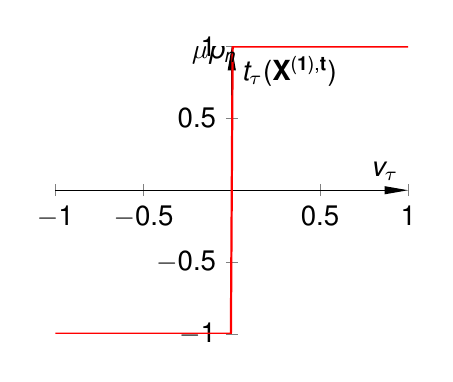
\begin{tikzpicture}
\begin{axis}[
%         grid= major ,
	  width=0.5\textwidth ,
	  xlabel style={font=\Large},
	  xlabel = {$v_\tau$} ,
	  ylabel style={font=\Large},
	  ylabel = {$t_\tau(\mathbf{X^{(1), t}})$} ,
	  xmin = -1,
	  xmax = 1,
	  ymin = -1,
	  ymax = 1,
	  axis lines=middle,
	  axis line style={myarrow}
	  ]
\addplot[red, thick] expression[domain=-1:1, domain y=-1:1, samples=200] {(x>0 ? 1 : -1)};
\node[] at (axis cs: -0.1,0.95) {$\mu p_n$};
\end{axis}
\end{tikzpicture}
\caption{\textit{Coulomb}'s schematic depiction of frictional contact conditions in tangential direction}
\label{fig:coulomb}
\end{center}
\end{figure}

The \textit{Coulomb}'s law can be defined as \eqref{eq:eqcoulomblaw}.

\begin{subequations}\label{eq:eqcoulomblaw}
\begin{equation}
\phi_{co} := \|\mathbf{t}_\tau \| - \mu \| p_n\| \leq 0 \label{eq:coul1}
\end{equation}
\begin{equation}
\mathbf{v}_{\tau, rel}(\mathbf{X}^{(1)}, t) + \beta \mathbf{t}_\tau = \mathbf{0} \label{eq:coul2}\\
\end{equation}
\begin{equation}
\beta \geq 0 \label{eq:coul3}
\end{equation}
\begin{equation}
\phi_{co} \beta = 0 \label{eq:coul4}
\end{equation}
\end{subequations}

Being $\mu$ the friction coefficient, and $\beta$ the velocity-traction ratio. Equation \eqref{eq:coul1} requires the magnitude of the tangential stress vector to not exceed the product of the coefficient of friction and the normal contact pressure. When the tangential stress is less than the \textit{Coulomb} limit ($\phi_{co} < 0$), the continuity equation \eqref{eq:coul4} forces the $\beta$ to be zero and, accordingly, the tangential relative velocity to be zero, this is called stick state. When the tangential stress is at the \textit{Coulomb} limit ($\phi_{co} = 0$)), $\beta$ may be greater than zero in \eqref{eq:coul4} and therefore the tangential stress is forced to oppose the relative tangential velocity in \eqref{eq:coul2}, this is called the slip state.

Finally the definition of the tangent direction is needed. We use the complementary direction to the normal, so calling the normal as $\mathbf{n}$ we can define the the tangent as \eqref{eq:tangentdefinition}.

\begin{subequations}\label{eq:tangentdefinition}
\begin{equation}
    \boldsymbol{\tau} = \mathbf{I} - \mathbf{n} \otimes \mathbf{n}
\end{equation}
With this we can define for example the tangent \textit{Lagrange} multiplier as:
\begin{equation}
    \boldsymbol{\lambda}_\tau = \boldsymbol{\lambda} - \mathbf{n} \lambda_n
\end{equation}
\end{subequations}

\subsubsection{Weak formulation}

\paragraph{Standard Lagrange multiplier}

The weak formulation of these equations can be obtained gain by multiplying \eqref{eq:eq0} with the test function $\mathbf{w}^{(i)} \in \mathcal{V}^{(i)}$ and integrating in each domain $i$ as \eqref{eq:eqweakfric}.

\begin{equation}\label{eq:eqweakfric}
\int_{\Omega_0^{(i)}}\left[ Div(\mathbf{F}^{(i)}\cdot \mathbf{S}^{(i)} + \hat{\mathbf{b}}_0^{(i)})\right] \cdot \mathbf{w}^{(i)} \text{d} \Omega_{0}^{(i)} + \int_{\Gamma_{\sigma}^{(i)}} \left[ \hat{\mathbf{t}}_0^{(i)} - \mathbf{P}^{(i)}\cdot \mathbf{N}^{(i)}  \right] \cdot \mathbf{w}^{(i)} \text{d} \Gamma_{\sigma}^{(i)} + \int_{\Gamma_{co}^{(i)}} \left[ \hat{\mathbf{t}}_{co,0}^{(i)} - \mathbf{P}^{(i)}\cdot \mathbf{N}^{(i)}  \right] \cdot \mathbf{w}^{(i)} \text{d} \Gamma_{co}^{(i)} = 0
\end{equation}

From \eqref{eq:eqweakfric} the part corresponding for the frictional contact would the shown in \eqref{eq:eqweakjustfric}.

\begin{equation}\label{eq:eqweakjustfric}
 \mathcal{W}^{co}(\mathbf{u},\boldsymbol{\lambda}) = \int_{\Gamma_c^{(1)}} \left[ \hat{\mathbf{t}}_{co,0}^{(i)} - \mathbf{P}^{(i)}\cdot \mathbf{N}^{(i)}  \right] \text{d}\Gamma_{co}^{(i)}
\end{equation}

If we consider the test function $\mathbf{w}^{(i)}$ as virtual displacements $\delta \mathbf{u}$, and with the application of the \textit{Gauss} divergence theorem it is possible to determine the equivalent expression for the virtual work \eqref{eq:eqvirtualfric}.

\begin{equation}\label{eq:eqvirtualfric}
\delta \mathcal{W}^{(i)}(\mathbf{u}^{(i)}, \delta \mathbf{u}^{i}) = \int_{\Omega_0^{(i)}} \mathbf{S}^{(i)} : \delta\mathbf{E}^{(i)}\text{d} \Omega^{(i)}_0 - \int_{\Omega_0^{(i)}}  \hat{\mathbf{b}}_0^{(i)} \cdot \delta \mathbf{u}^{(i)}\text{d} \Omega_0^{(i)} - \int_{\Sigma_{\sigma}^{(i)}}\hat{\mathbf{t}}_0^{(i)} \cdot \delta \mathbf{u}^{(i)}\text{d}\Gamma_{\sigma}^{(i)} - \int_{\Gamma_{co}^{(i)}}\mathbf{t}_{co,0}^{(i)}\cdot \delta \mathbf{u}^{(i)}\text{d}\Gamma_{co}^{(i)} = 0 \forall \delta \mathbf{u}^{i} \in \mathcal{V}^{(i)}
\end{equation}

Equation \eqref{eq:eqvirtualfric} can be regrouped on contributions as in \eqref{eq:constributions}, obtaining \eqref{eq:constributionsfric}.

\begin{subequations}\label{eq:constributionsfric}
 \begin{align}
  & -\delta \mathcal{W}_{kin} = \sum_{i = 1}^2 \left[\int_{\Omega_0^{(i)}} \rho_0^{(i)} \ddot{\mathbf{u}}^{(i)} \cdot \delta \mathbf{u}^{(i)} \text{d}\Omega_{0}^{(i)}\right] \label{eq:subeq10fric} \\
 & -\delta \mathcal{W}_{int,ext} = \sum_{i = 1}^2 \left[\int_{\Omega_0^{(i)}} \left(\mathbf{S}^{(i)} : \delta \mathbf{E}^{(i)} - \hat{\mathbf{b}}\cdot \delta\mathbf{u}^{(i)} \right) \text{d}\Omega_{0}^{(i)} - \int_{\Gamma_\sigma^{(i)}} \hat{\mathbf{t}}_0^{(i)}\cdot\delta\mathbf{u}^{(i)} \text{d}\text{d} \Gamma_{\sigma}^{(i)} \right] \label{eq:subeq11fric} \\
 & -\delta \mathcal{W}_{co} = \sum_{i = 1}^2 \left[\int_{\Gamma_{co}^{(i)}} \mathbf{t}_{co}^{(i)} \cdot \delta \mathbf{t}_c^{(i)} \text{d}\Gamma_{co}^{(i)}\right] \label{eq:subeq12fric}
 \end{align}
\end{subequations}

 Where $\mathbf{t}_{co}$ represents the traction on the interface, the balance between the contact interface implies \eqref{eq:traction}

\begin{equation}\label{eq:traction}
\mathbf{t}_{co}^{(1)} \text{d}\gamma^{(1)} = -\mathbf{t}_{co}^{(2)} \text{d}\gamma^{(2)}
\end{equation}

As in the frictionless case we will take the slave surface as reference, this allows to rewrite the virtual work integral for the contact as \eqref{eq:virtualcontact}.

\begin{subequations}\label{eq:constributionsfric}
\begin{equation}\label{eq:virtualcontact}
\delta \mathcal{W}_{co} = - \int_{\Gamma_{co}^{(1)}} \mathbf{t}_{co}^{(1)} \cdot \delta g \text{d}\Gamma_{co}^{(1)}
\end{equation}
 Where $g$ represents the general gap \eqref{eq:eqgeneralgap} (instead of just normal gap).
\begin{equation}\label{eq:eqgeneralgap}
 g= \left( \mathbf{u}^{(1)} - \chi \cdot \mathbf{u}^{(2)}\right)
\end{equation}
The \textit{Lagrange} multiplier are introduced as additional unknowns on the slave contact surface and are identified as the
negative contact traction as \eqref{eq:lm}.
\begin{equation}\label{eq:lm}
    \boldsymbol{\lambda} = - \mathbf{t}_{co}^{(1)}
\end{equation}
\end{subequations}

\paragraph{Contact constrains}

The Equation \eqref{eq:virtualcontact} is reformulated. Using the \textit{Lagrange} multiplier in \eqref{eq:lm} we can decompose into normal and tangential components $\lambda_n$ and $\boldsymbol{\lambda}_\tau$ \eqref{eq:eqdecomp}.

\begin{subequations}\label{eq:eqdecomp}
\begin{equation}
\lambda_n \in \mathds{R}_0^{+}: g (\delta \lambda_n - \lambda_n) \geq 0 \forall \delta \lambda_n \in \mathds{R}_0^{+}
\end{equation}
\begin{equation}
\boldsymbol{\lambda}_\tau \in \mathcal{B}(\mu \lambda_n): \mathbf{v}_{\tau,rel} \cdot (\delta \boldsymbol{\lambda}_\tau - \boldsymbol{\lambda}_\tau) \leq 0 \forall \delta \boldsymbol{\lambda}_\tau \in \mathcal{B}(\mu \lambda_n)
\end{equation}
\end{subequations}

Where $\mathcal{B}(\mu \lambda_n)$ is a $(n − 1)$-dimensional sphere with centre 0 and radius $\mu \lambda_n$ and $\boldsymbol{\lambda}_\tau$ is a \emph{trial} force in the tangential plane. It is the so-called principle of maximal dissipation representing \textit{Coulomb}'s law of friction.

Then  \eqref{eq:virtualcontact} can be rewritten and the weak form of both normal and tangential contact conditions is obtained as \eqref{eq:eqfrictionalcontact}.

\begin{subequations}\label{eq:eqfrictionalcontact}
\begin{equation}
\boldsymbol{\lambda} \in \mathcal{M}(\boldsymbol{\lambda}) : \int_{\lambda_{co}^{(1)}} g (\delta \lambda_n - \lambda_n) d \lambda \geq 0,
\end{equation}
\begin{equation}
\int_{\lambda_{co}^{(1)}} \mathbf{v}_{\tau,rel} (\delta \boldsymbol{\lambda}_\tau - \boldsymbol{\lambda}_\tau) d \lambda \leq 0 \forall \delta \boldsymbol{\lambda} \in \mathcal{M}(\boldsymbol{\lambda})
\end{equation}
\end{subequations}

Where $ \mathcal{M}(\boldsymbol{\lambda})$ is the admissible solution space for the \textit{Lagrange} multiplier and the test space for the trial force $\delta \boldsymbol{\lambda}$. It is a convex subset $ \mathcal{M}(\boldsymbol{\lambda}) \subset \mathcal{M}$ which accommodates the restrictions of $\boldsymbol{\lambda}$ and $\delta \boldsymbol{\lambda}$ in \eqref{eq:eqdecomp}. The subspace can be rewritten as \eqref{eq:subspace}.

\begin{equation}\label{eq:subspace}
    \mathcal{M}(\boldsymbol{\lambda}) := \left\{ \delta \boldsymbol{\lambda} \in  \mathcal{M} : \langle \delta \boldsymbol{\lambda}, \boldsymbol{\eta} \rangle \leq \langle \mu \lambda_n, \| \boldsymbol{\eta}_\tau \| \rangle, \boldsymbol{\eta} \in \mathcal{W}^{(1)} with \eta_n \leq 0 \right\}
\end{equation}

Here $\langle \cdot, \cdot \rangle$ is the duality pairing of the spaces $\mathcal{M}$ and $\mathcal{V}^{(1)}$ on $\gamma_{co}^{(1)}$ given by \eqref{eq:pairing}.

\begin{equation}\label{eq:pairing}
\langle \delta \boldsymbol{\lambda}, \boldsymbol{\eta} \rangle := \int_{\gamma_{co}^{(1)}} \delta \boldsymbol{\lambda} \boldsymbol{\eta} d \gamma
\end{equation}

\paragraph{Augmented Lagrange multiplier}

In the very same way we have defined an \textbf{Augmented Lagrangian} for the frictionless method we can define the same for the frictional case. The \textbf{Augmented Lagrangian} method to solve contact problems with friction was proposed by \textit{Alart and Curnier}\cite{alart}, additionally to these references we have considered the work of \textit{Cardona}\cite{cardona3} and \textit{Yastrebov}\cite{yastrebov}.

Focusing in the functional relative to the contact ($\mathcal{W}^{co}(\mathbf{u},\boldsymbol{\lambda)} = \mathcal{W}^{co}_\mathcal{V} + \mathcal{W}_\mathcal{M}$), we can rewrite \eqref{eq:eqweakjustfric} as \eqref{eq:eqalmfunctfrictional0}.

\begin{equation}\label{eq:eqalmfunctfrictional0}
 \mathcal{W}^{co}(\mathbf{u},\boldsymbol{\lambda}) = \int_{\Gamma_c^{(1)}} l_n + l_\tau \text{d}\Gamma_{co}^{(i)}
\end{equation}

Being $l_n$ and $l_\tau$ \eqref{eq:eqlnlt} the corresponding parts of the \textit{Augmented Lagrangian} formulation for the normal and tangent contributions respectively.

\begin{subequations}\label{eq:eqlnlt}
\begin{equation}
l_n(g_n,\lambda_n) = \begin{cases} \hat{\lambda}_n g_n - \frac{\varepsilon_n}{2} g_n^2 \text{ , } \hat{\lambda}_n \leq 0 \text{, contact} \\ -\frac{k^2}{2\varepsilon_n}\lambda_n^2 \text{ , } \hat{\lambda}_n > 0 \text{, non contact} \end{cases}
\end{equation}
With $\hat{\lambda}_n= k \lambda_n +\varepsilon_n \g_n$ being the augmented \textit{Lagrange} multiplier for the normal direction.
\begin{equation}
l_\tau(\mathbf{v}_{\tau, rel}, \boldsymbol{\lambda}_\tau) = \begin{cases} \begin{cases} \hat{\boldsymbol{\lambda}}_\tau \cdot \mathbf{v}_{\tau, rel} - \frac{\varepsilon_\tau}{2} \mathbf{v}_{\tau, rel} \cdot \mathbf{v}_{\tau, rel} & \text{, } \| \hat{\boldsymbol{\lambda}}_\tau \| \leq - \mu \hat{\lambda}_n \text{, stick} \\ -\frac{1}{2\varepsilon_\tau} \left(k^2  \boldsymbol{\lambda}_\tau \cdot \boldsymbol{\lambda}_\tau  + 2 \mu \hat{\lambda}_n \| \boldsymbol{\lambda}_\tau \| + \mu^2 + \hat{\lambda}_n^2 \right) & \text{, } \| \hat{\boldsymbol{\lambda}}_\tau \| > - \mu \hat{\lambda}_n \text{, slip}  \end{cases} & \text{ , } \hat{\lambda}_n \leq 0 \text{, contact} \\  -\frac{k^2}{2\varepsilon_\tau}\boldsymbol{\lambda_\tau} \cdot \boldsymbol{\lambda_\tau} & \text{ , } \hat{\lambda}_n > 0 \text{, non contact}   \end{cases}
\end{equation}
With $\hat{\boldsymbol{\lambda}}_\tau= k \boldsymbol{\lambda}_\tau + \varepsilon_\tau \mathbf{v}_{\tau, rel}$ being the augmented \textit{Lagrange} multiplier for the tangent direction.
\end{subequations}

Where $\varepsilon_n$ and $\varepsilon_\tau$ are a positive penalty parameter, both for normal and tangent direction, $k$ is a positive scale factor. Using the $\langle \rangle$ is the \textit{Macauley} bracket operator, from \eqref{eq:eqmac}, we can express everything as \eqref{eq:eqlnltmaca}.

\begin{subequations}\label{eq:eqlnltmaca}
\begin{equation}
l_n(g_n,\lambda_n) = \frac{1}{\varepsilon_n} \left(k^2 \lambda_n^2 - \langle \hat{\lambda}_n \rangle^2 \right)
\end{equation}
\begin{equation}
l_\tau(\mathbf{v}_{\tau, rel}, \boldsymbol{\lambda}_\tau) = \frac{1}{\varepsilon_\tau} \left(k^2 \boldsymbol{\lambda}_\tau \cdot \boldsymbol{\lambda}_\tau -\| \hat{\boldsymbol{\lambda}}_\tau \|^2 - \langle \| \hat{\boldsymbol{\lambda}}_\tau \| - \mu \| - \hat{\lambda}_n \| \rangle^2 \right)
\end{equation}
\end{subequations}

This functional is $\mathcal{C}^1$ differentiable saddle-point, as shown in Figure \ref{fig:locusalmfrictional}. The solution is obtained as the set of values that render this functional stationary.

\begin{figure}[h]
\begin{center}
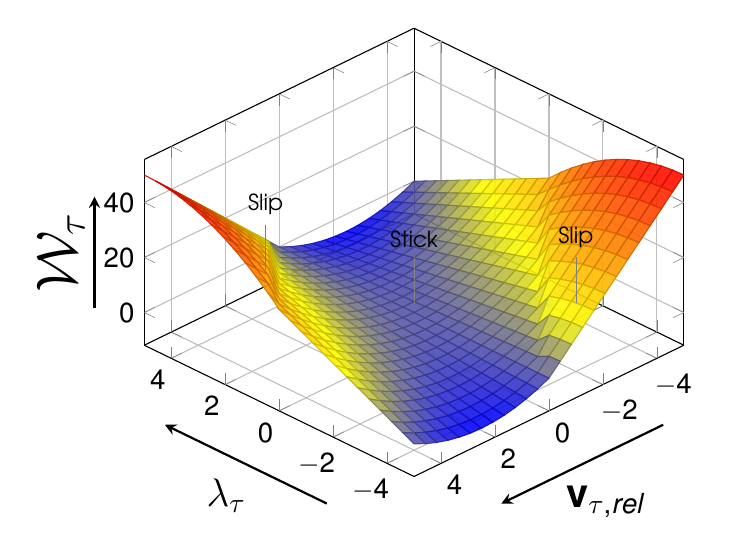
\begin{tikzpicture}[
declare function={functional(\ln,\mu)={(\ln > 0 ? (\ln)^2 + (x)^2 : abs(x+y) > - (\mu * \ln) ? - (x^2 + 2 * \mu * \ln * abs(x + y) + \mu^2 * \ln^2 ) : x*y + y^2 )};}
]
\begin{axis}[grid=both,
%             title= Augmented Lagrangian function for the contact problem,
            xlabel={$\lambda_\tau$},
            xticklabel pos=left,
            xlabel style={font=\Large},
            ylabel={$\mathbf{v}_{\tau, rel}$},
            x dir=reverse,
            yticklabel pos=left,
            ylabel style={font=\Large},
            y dir=reverse,
            zlabel={$\mathcal{W}_\tau$},
            zticklabel pos=left,
            zlabel style={font=\huge},
%             xmin=-20,
%             xmax=20,
%             ymin=-20,
%             ymax=20,
%             zmin=-600,
%             zmax=600,
            after end axis/.code={
                \draw [-stealth, thick, black] (xticklabel cs:0.8) -- (xticklabel cs:0.2);
                \draw [-stealth, thick, black] (yticklabel cs:0.8) -- (yticklabel cs:0.2);
                \draw [-stealth, thick, black] (zticklabel cs:0.2) -- (zticklabel cs:0.8);
            }
            ,unbounded coords = jump
            ,view = {45}{45}
%             ,colormap name  = whitered
%             ,colorbar style = {
%                 at     = {(1,0)},
%                 anchor = south west,
%                 height = 0.25*\pgfkeysvalueof{/pgfplots/parent axis height},
%                 title  = {$\mathcal{W}$}
%                 }
            ]
\addplot3[surf,opacity=0.9,shader=faceted]{functional(-1.0,5.0)};
% \addplot3[samples=30, domain=-20:0, samples y=0, thick,red,smooth]({-5},{x},0});
% \addplot3[samples=30, domain= -5:5,samples y=0, thick,red,smooth]({x},{0.0},{0.0});
% \addplot3[samples=30, domain= 0:20,samples y=0, thick,red,smooth]({5},{x},0);
\node at (axis cs: 4.0,1.5,0.0 ) [pin=90:\footnotesize{Slip}] {};
\node at (axis cs: -3.0,-3.0,0.0 ) [pin=90:\footnotesize{Slip}] {};
\node at (axis cs: 0.0,0.0,0.0 ) [pin=90:\footnotesize{Stick}] {};
\end{axis}
\end{tikzpicture}
\caption{Augmented Lagrangian function for the frictional contact problem}
\label{fig:locusalmfrictional}
\end{center}
\end{figure}

As in the frictionless case he solution does not depend on the value of parameters $\varepsilon$ and $k$. Nevertheless, the convergence rate does depend on their value. Finally we can derive \eqref{eq:eqalmfunctfrictional0} to obtain the variational form from \eqref{eq:eqalmfunctfrictional}.

\begin{equation}\label{eq:eqalmfunctfrictional}
  \delta \mathcal{W}^{co}(\mathbf{u},\boldsymbol{\lambda}) = \int_{\Gamma_c^{(1)}}\begin{cases}  \hat{\lambda}_{n} \cdot \delta g_n + k g_n \delta\lambda_n + \hat{\boldsymbol{\lambda}}_\tau \cdot \delta \mathbf{v}_{\tau, rel} + \mathbf{v}_{\tau, rel} \cdot \delta \hat{\boldsymbol{\lambda}}_\tau & \text{ if } \| \hat{\boldsymbol{\lambda}}_{\tau} \| \leq -\mu \hat{\lambda}_{n}  \text{ (Contact stick zone)}
  \\ \hat{\lambda}_{n} \cdot \delta g_n + k g_n \delta\lambda_n - \mu  \hat{\lambda}_{n}  * \frac{\hat{\boldsymbol{\lambda}}_{\tau} }{\| \hat{\boldsymbol{\lambda}}_{\tau} \|} - \frac{1}{\varepsilon_\tau} \left( k  \boldsymbol{\lambda}_{\tau} + \mu  \hat{\lambda}_{n} \frac{\hat{\boldsymbol{\lambda}}_{\tau} }{\| \hat{\boldsymbol{\lambda}}_{\tau} \|} \right) \delta\boldsymbol{\lambda}_{\tau} & \text{ if } \| \hat{\boldsymbol{\lambda}}_{\tau} \| > - \mu \hat{\lambda}_{n}  \text{ (Contact slip zone)}
  \\  - \frac{k^2}{\varepsilon_n} \lambda_n \delta\lambda_n - \frac{k^2}{\varepsilon_\tau} \boldsymbol{\lambda}_{\tau} \delta\boldsymbol{\lambda}_{\tau}& \text{ if } \hat{\lambda}_{n} > 0 \text{ (Gap zone)} \end{cases} \text{d}\Gamma_{co}^{(i)}
\end{equation}

The functional from \eqref{eq:eqalmfunctfrictional} makes that the system obtained varies in function if the nodes are present in the contact(slip or stick) or the gap zone, the system is not a priori known like in the frictionless case but with and additional configuration.

\subsubsection{Discretisation and numerical integration}

Many of the things defined for the frictionless case, like the definition of the dual \textit{Lagrange} multipliers or the definition of the mortar operators remain exactly the same. In this case we will focus in the kinematic definitions for the frictional case using the mortar operators, basically the definition of the discrete contact condition in the tangential direction and the slip in the discrete using the mortar operators.

\paragraph{Discrete contact condition in tangential direction}

Following the same procedure for the normal direction we can obtain the part equivalent for the tangential direction. The most relevant thing to take into account before any definition is the concept of the relative velocity in the tangential direction $\mathbf{v}_{\tau, rel}$ , where we will use for our definition the discrete form of the material velocity field $\dot{\mathbf{x}}^{(i)}$, which uses the same shape functions for interpolation as the $\mathbf{x}^{(i)}$. We can then define \eqref{eq:eqfrictionalcontactdiscrete}.

\begin{equation}\label{eq:eqfrictionalcontactdiscrete}
\begin{aligned}
& \int_{\gamma_c^{(1)}} \mathbf{v}_{\tau, vel} \cdot \left( \delta \boldsymbol{\lambda}_\tau - \boldsymbol{\lambda}_\tau \right) d\gamma \\ & \approx \sum_{j=1}^{n_{slaves}} \left( \delta \boldsymbol{\lambda}_\tau - \boldsymbol{\lambda}_\tau \right)^T \boldsymbol{\tau}_j \left[ \int_{\gamma_c^{(1)}} \Phi_j N_j^{(1)} d\gamma \dot{\mathbf{x}}_j^{(1)} - \sum_{l=1}^{n_{master}} \int_{\gamma_c^{(1)}} \Phi_j \left(N_l^{(2)} \cdot \xi \right) d\gamma \dot{\mathbf{x}}_l^{(2)} \right] \geq 0 \forall \delta \boldsymbol{\lambda} \in \mathcal{M}(\boldsymbol{\lambda})
\end{aligned}
\end{equation}

We can express this equation using the mortar operators, see \ref{section:mortar}, what will give us the following expression \eqref{eq:eqfrictionalcontactdiscreteoperators}.

\begin{equation}\label{eq:eqfrictionalcontactdiscreteoperators}
 \int_{\gamma_c^{(1)}} \mathbf{v}_{\tau, vel} \cdot \left( \delta \boldsymbol{\lambda}_\tau - \boldsymbol{\lambda}_\tau \right) d\gamma \approx \sum_{j=1}^{n_{slaves}} \left( \delta \boldsymbol{\lambda}_\tau - \boldsymbol{\lambda}_\tau \right)^T \boldsymbol{\tau}_j \left[\mathbf{D}_{j} \dot{\mathbf{x}}_j^{(1)} - \sum_{l=1}^{n_{master}} \mathbf{M}_{l} \dot{\mathbf{x}}_l^{(2)} \right] =  \sum_{j=1}^{n_{slaves}} \left( \delta \boldsymbol{\lambda}_\tau - \boldsymbol{\lambda}_\tau \right)^T \tilde{\mathbf{v}}_{\tau j} \geq 0
\end{equation}

Where $\tilde{\mathbf{v}}_{\tau j}$ is the weighted relative velocity.

\paragraph{Slip definition}

An important aspect of a proper formulation of frictional laws in the finite sliding context is frame indifference\cite{gitt1, laursen2} of the rate measures involved. This affects the tangential relative velocity of the contacting bodies $\mathbf{v}_{\tau, rel}$ in the considered case of frictional contact. This assures that this quantity is unaffected by any rigid body motion which the two contacting bodies might experience at the instant of question. Mathematically, this can be tested with formulating the tangential relative velocity $\mathbf{v}_{\tau rel}$  in an alternative reference frame. Then in the current (mortar projected) instance, we must ensure frame indifference.

Working in the time continuous case first, one may readily show that the tangential component of the mortar projected tangential velocity is not frame indifferent:

\begin{subequations}
\begin{equation}\label{eq:eqobj2}
\tilde{\mathbf{v}}_{\tau}^{nononbj} =  \boldsymbol{\tau}_j \left[\mathbf{D}_{j} \dot{\mathbf{x}}_j^{(1)} - \sum_{l=1}^{n_{master}} \mathbf{M}_{l} \dot{\mathbf{x}}_l^{(2)} \right]
\end{equation}
Frame indifference is assessed by viewing the motion from another reference frame, denotes in the following by superscripts $∗$ , which can be related to the original spatial frame via:
\begin{equation}\label{eq:eqobj1}
\dot{\mathbf{x}}_l^{(1*)} = \mathbf{c}(t) + \mathbf{Q}(t) \dot{\mathbf{x}}_l^{(1)}
\end{equation}
Where $\mathbf{c(t)}$ is the relative rigid body translation between the original spatial frame and observer $*$, while a relative rotation is produced by the proper orthogonal tensor $\mathbf{Q}(t)$. The frame indifferent relative tangential velocity should satisfy.
\begin{equation}
\tilde{\mathbf{v}}_{\tau}^{*} = \mathbf{Q}(t)\tilde{\mathbf{v}}_{\tau}
\end{equation}
However, by considering the effect of the transformation \eqref{eq:eqobj1} on \eqref{eq:eqobj2}, it is readily seen that:
\begin{equation}
\tilde{\mathbf{v}}_{\tau}^{nonobj*} = \mathbf{Q}(t)\tilde{\mathbf{v}}_{\tau}^{nonobj} - \dot{\mathbf{Q}}(t) \mathbf{Q}\boldsymbol{\tau}_j  \left[\mathbf{D}_{j} \mathbf{x}_j^{(1)} - \sum_{l=1}^{n_{master}} \mathbf{M}_{l} \mathbf{x}_l^{(2)} \right]
\end{equation}
Because the term $\left[\mathbf{D}_{j} \mathbf{x}_j^{(1)} - \sum_{l=1}^{n_{master}} \mathbf{M}_{l} \mathbf{x}_l^{(2)} \right]  \neq \mathbf{0}$ in general $\tilde{\mathbf{v}}_{\tau}^{nonobj*}$ does not satisfy the equation , and thus some modifications are required to this relative velocity measure to assure material frame indifference. It is possible to restore the objectivity with the inclusion of the rate of a mortar projected distance between the two bodies, denoted as $\mathbf{g}$. Then in consequence:
\begin{equation}\label{eq:objective1}
\tilde{\mathbf{v}}_{\tau} = \boldsymbol{\tau}_j \left[\mathbf{D}_{j} \dot{\mathbf{x}}_j^{(1)} - \sum_{l=1}^{n_{master}} \mathbf{M}_{l} \dot{\mathbf{x}}_l^{(2)} - \dot{\mathbf{g}} \right]
\end{equation}
We obtain an expression which retains the interpretation of the tangential relative velocity in the case where perfect sliding occurs (i.e. when $ \dot{\mathbf{g}}=0$), but which contains the modification necessary to make the velocity measure objective under all conditions of contact. This is readily seen by using direct calculation to exactly reexpress \eqref{eq:objective1} as \eqref{eq:objective2}, considering \eqref{eq:objective1b}.
\begin{equation}\label{eq:objective1b}
    \dot{\mathbf{g}} = \frac{\text{d}}{\text{d}t} \left[\dot{\mathbf{D}}_{j} \mathbf{x}_j^{(1)} - \sum_{l=1}^{n_{master}} \dot{\mathbf{M}}_{l} \mathbf{x}_l^{(2)} \right] = \left[\dot{\mathbf{D}}_{j} \dot{\mathbf{x}}_j^{(1)} - \sum_{l=1}^{n_{master}} \dot{\mathbf{M}}_{l} \dot{\mathbf{x}}_l^{(2)} \right] + \left[\dot{\mathbf{D}}_{j} \mathbf{x}_j^{(1)} - \sum_{l=1}^{n_{master}} \dot{\mathbf{M}}_{l} \mathbf{x}_l^{(2)} \right]
\end{equation}
\begin{equation}\label{eq:objective2}
\tilde{\mathbf{v}}_{\tau} = \boldsymbol{\tau}_j \left[\dot{\mathbf{D}}_{j} \mathbf{x}_j^{(1)} - \sum_{l=1}^{n_{master}} \dot{\mathbf{M}}_{l} \mathbf{x}_l^{(2)} \right]
\end{equation}
\end{subequations}

The time derivatives of the mortar operators can be defined using any desired scheme, for example using the \textit{backward Euler}\eqref{eq:eqeuler} scheme as time discretization.

\begin{subequations}\label{eq:eqeuler}
\begin{equation}
\frac{\text{d} \left(\cdot\right)}{\text{d}t} \approx \frac{\left(\cdot\right)^{t+\Delta t} - \left(\cdot\right)^{t}}{\Delta t}
\end{equation}
\begin{equation}
\frac{\text{d} \mathbf{D}}{\text{d}t} \approx \frac{\mathbf{D}_l^{t+\Delta t} - \mathbf{D}_j^{t}}{\Delta t} \text{, } \frac{\text{d} \mathbf{M}}{\text{d}t} \approx \frac{\mathbf{M}_l^{t+\Delta t} - \mathbf{M}_l^{t}}{\Delta t}
\end{equation}
\end{subequations}

With this we can define  tangential relative velocity $\tilde{\mathbf{v}}_{\tau}$  as \eqref{eq:objective2withdelta}, that multiplies by $\Delta t$ gives us the nodal slip increment $\tilde{\mathbf{u}}_{\tau}$ \eqref{eq:objective2withdeltafinal}.

\begin{equation}\label{eq:objective2withdelta}
\tilde{\mathbf{v}}_{\tau} = \boldsymbol{\tau}_j \left[ \frac{\mathbf{D}_j^{t+\Delta t} - \mathbf{D}_j^{t}}{\Delta t} \mathbf{x}_j^{(1)} - \sum_{l=1}^{n_{master}} \frac{\mathbf{M}_l^{t+\Delta t} - \mathbf{M}_l^{t}}{\Delta t} \dot{\mathbf{x}}_l^{(2)} \right]
\end{equation}
\begin{equation}\label{eq:objective2withdeltafinal}
\tilde{\mathbf{u}}_{\tau} = \boldsymbol{\tau}_j \left[ \left(\mathbf{D}_j^{t+\Delta t} - \mathbf{D}_j^{t}\right) \mathbf{x}_j^{(1)} - \sum_{l=1}^{n_{master}} \left(\mathbf{M}_l^{t+\Delta t} - \mathbf{M}_l^{t}\right) \dot{\mathbf{x}}_l^{(2)} \right]
\end{equation}

\paragraph{Matrix form of the problem}

\textcolor{red}{Complete with all the casuistry }

\subsubsection{Active set strategy (Semismoth Newton Raphson)}

The reformulation of frictional contact conditions is similar to the frictionless case. It takes the form of a two component vector equation and is written as \eqref{eq:eqcompfrictional}, the visual representation can be seen in Figure \ref{fig:complemenrary_frictional}.

\begin{equation}\label{eq:eqcompfrictional}
\mathbf{C}_{\tau j}(\boldsymbol{\lambda}_\tau, \tilde{\mathbf{u}}_{\tau}) = max(\mu \tilde{\lambda}_n, \| \tilde{\boldsymbol{\lambda}}_\tau \|) \boldsymbol{\lambda}_\tau - \mu max(0, \lambda_n)\tilde{\boldsymbol{\lambda}}_\tau
\end{equation}

\begin{figure}[h]
\begin{center}
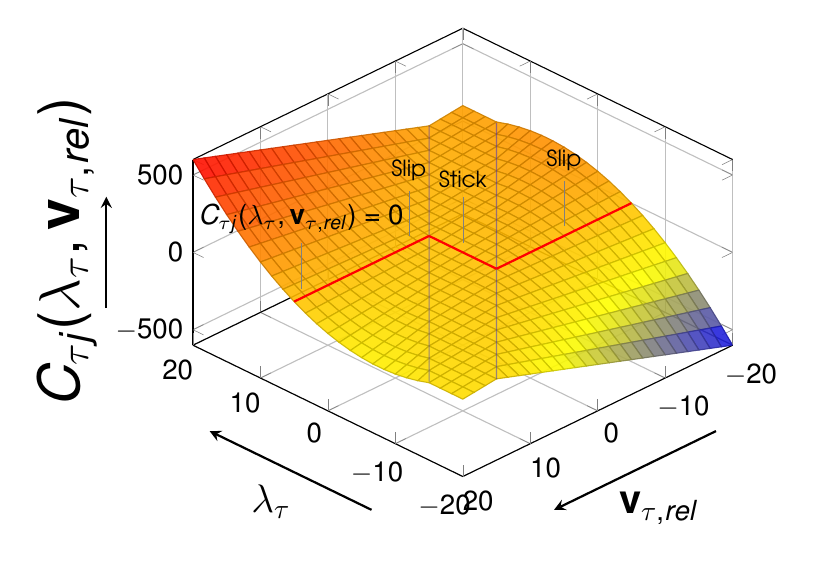
\begin{tikzpicture}[
declare function={myfunction(\ln,\mu)={(max(\mu * \ln, abs(x + y)) * x - \mu * max(0, \ln) * (y+x))};}
]
\begin{axis}[grid=both,
            xlabel={$\lambda_\tau$},
            xticklabel pos=left,
            xlabel style={font=\Large},
            ylabel={$\mathbf{v}_{\tau, rel}$},
            yticklabel pos=left,
            ylabel style={font=\Large},
            zlabel={$C_{\tau j}(\lambda_\tau, \mathbf{v}_{\tau, rel})$},
            zticklabel pos=left,
            zlabel style={font=\huge},
            x dir=reverse,
            y dir=reverse,
            xmin=-20,
            xmax=20,
            ymin=-20,
            ymax=20,
            zmin=-600,
            zmax=600,
            after end axis/.code={
                \draw [-stealth, thick, black] (xticklabel cs:0.8) -- (xticklabel cs:0.2);
                \draw [-stealth, thick, black] (yticklabel cs:0.8) -- (yticklabel cs:0.2);
                \draw [-stealth, thick, black] (zticklabel cs:0.2) -- (zticklabel cs:0.8);
            }
            ,unbounded coords = jump
            ,view = {45}{45}
            ]
\addplot3[surf,opacity=0.9,shader=faceted,domain=-20:20,domain y=-20:20]{myfunction(1.0, 5.0)};
\addplot3[samples=30,opacity=0.4, domain=-16.8:22.2, samples y=0,blue,smooth]({-5+x},{-x},{0.0});
\addplot3[samples=30,opacity=0.4, domain=-22.2:16.8, samples y=0,blue,smooth]({5+x},{-x},{0.0});
\addplot3[samples=30, domain=-20:0, samples y=0, thick,red,smooth]({-5},{x},{0.0});
\addplot3[samples=30, domain= -5:5,samples y=0, thick,red,smooth]({x},{0.0},{0.0});
\addplot3[samples=30, domain= 0:20,samples y=0, thick,red,smooth]({5},{x},{0.0});
\node at (axis cs: 5.0,19.0,0.0 ) [pin=90:\normalsize{$C_{\tau j}(\lambda_\tau, \mathbf{v}_{\tau, rel}) = 0$}] {};
\node at (axis cs: 5.0,3.0,0.0 ) [pin=90:\footnotesize{Slip}] {};
\node at (axis cs: -5.0,-10.0,0.0 ) [pin=90:\footnotesize{Slip}] {};
\node at (axis cs: 0.0,0.0,0.0 ) [pin=90:\footnotesize{Stick}] {};
\end{axis}
\end{tikzpicture}
\caption{Complementary function for the frictional contact problem.}
\label{fig:complemenrary_frictional}
\end{center}
\end{figure}

\begin{thebibliography}{99}

\bibitem{popp1} Popp, Alexander {\em Mortar Methods for Computational Contact Mechanics and General Interface Problems}  2012.

\bibitem{popp2}  Popp, Alexander and Gitterle, Markus and Gee, Michael W. and Wall, Wolfgang A. {\em A dual mortar approach for 3D finite deformation contact with consistent linearization} 2010: International Journal for Numerical Methods in Engineering

\bibitem{gitt1} Gitterle, Markus,{\em A dual mortar formulation for finite deformation frictional contact problems including wear and thermal coupling}, 2012.

\bibitem{doca1} Doca, Thiago de Carvalho Rodrigues,{\em Energy wear methods for dual-mortar contact analysis of frictional problems at finite inelastic strains}, 2014.

\bibitem{doca2} Doca, Thiago de Carvalho Rodrigues,{\em A frictional mortar contact approach for the analysis of large inelastic deformation problems}, 2014.

\bibitem{laursen1} Laursen, Tod A, Puso, Michael A and Sanders, Jessica {\em Mortar contact formulations for deformable–deformable contact: past contributions and new extensions for enriched and embedded interface formulations}, 2012.

\bibitem{laursen2} Yang, Bin, Laursen, Tod A, Puso and Meng, Xiaonong {\em Two dimensional mortar contact methods for large deformation frictional sliding}, 2005.

\bibitem{alart}   Alart P, Curnier A.  {\em A mixed formulation for frictional contact problems prone to Newton like solution methods.} 1991: Computer Methods in Applied Mechanics and Engineering; 92:353–375.

\bibitem{yastrebov} Yastrebov, Vladislav A. {\em Computational contact mechanics: geometry, detection and numerical techniques}, 2011

\bibitem{cardona1}  Calavalieri, FJ and Cardona, Alberto {\em An augumented lagrangian method to solve three-dimensional nonlinear contact problems} 2012: Latin American applied research

\bibitem{cardona2}  Calavalieri, FJ and Cardona, Alberto {\em An augmented Lagrangian technique combined with a mortar algorithm for modelling mechanical contact problems} 2013: International Journal for Numerical Methods in Engineering

\bibitem{cardona3}  Calavalieri, FJ and Cardona, Alberto {\em Numerical solution of frictional contact problems based on a mortar algorithm with an augmented Lagrangian technique} 2015: Multibody System Dynamics

\bibitem{wohlmuth} B. I. Wohlmuth,{\em Discretization methods and iterative solvers based on domain decomposition}, Springer-Verlag Berlin Heidelberg, 2001.

\bibitem{Zienkiewicz1} Zienkiewicz, O. C. and Zhu, J.Z. and Taylor, Robert L.,{\em The Finite Element Method: its Basis and Fundamentals}, Butterworth-Heinemann, 2013.

\end{thebibliography}

\end{document}
